%&latex
\documentclass[letterpaper]{article}
\usepackage{aaai}
\usepackage{amsfonts}
\usepackage{times}
\usepackage{helvet}
\usepackage{courier}
\usepackage{ifthen}

\nocopyright

\newcommand{\fix}[1]{{$\langle${\sc #1}$\rangle$}}

\usepackage[pdftex]{graphicx}
\usepackage{amsmath}

\newcounter{codeline}
\newenvironment{code}{
  \newcommand{\cl}{ % code line
    \refstepcounter{codeline}
    \ifthenelse{\value{codeline}<10}{\hspace{5pt}\arabic{codeline}}{\arabic{codeline}}.
  }
  \begin{tabbing}
    00. nn\=nn\=nn\=nn\=nn\=nn\=nn\=nn\=nn\=nn\kill
} {\end{tabbing}}

% italics in math mode
\newcommand{\myit}[1]{\mbox{\em #1}}
% in subscripts
\newcommand{\myits}[1]{\mbox{\scriptsize \em #1}}

\newcommand{\citep}[1]{\citeauthor{#1}~\shortcite{#1}}
\newcommand{\citeq}[1]{\citeauthor{#1}~\citeyear{#1}}

\newcommand{\fromM}[1]{{$\langle${\sc M: #1}$\rangle$}}
\newcommand{\pv}{\myit{PlanVisioner }}

% evil
\def\baselinestretch{.968}
\setlength\textheight{9.12in}
%\setlength\textwidth{7.1in}
\setlength\columnsep{0.245in}

\newcommand{\figwidth}[2]{\mbox{\resizebox{#1}{!}
{\includegraphics{#2}}}}

\newcommand{\fixE}[1]{$\langle${\sc EB: #1}$\rangle$}

%------------------------------
\begin{document}

\title{EUROPA: A Platform for AI Planning, Scheduling, Constraint Programming, and Optimization}


\author{Javier Barreiro, Tristan Smith, Paul Morris, Jeremy Frank, \\ add\_some\_people\_here (Ari, Conor, Michael?), Minh Do}

%Keywords: Planning, real-time}


\date{}
\maketitle

%------
\begin{abstract}

EUROPA is a class library and tool set for building planners (and/or schedulers) within a Constraint-based Temporal Planning paradigm. This paradigm has been successfully applied in a wide range of practical planning problems and has a legacy of success in NASA applications. EUROPA offers capabilities in 3 key areas of problem solving: (1) Representation; (2) Reasoning; and (3) Search. EUROPA is a mean to integrate advanced planning, scheduling and constraint reasoning into an end-user application and is designed to be open and extendable to accommodate diverse and highly specialized problem solving techniques within a common design framework and around a common technology core.  In this paper, we will demonstrate the core capabilities of this open-source planning \& scheduling framework and our development roadmap for EUROPA. While EUROPA is the complete planning and scheduling software suite, we will concentrate on the aspects that are relevant to the knowledge engineering purpose: modeling language capabilities, model debugging and execution tools, and plan visualization and analysis.

\end{abstract}
%-----


%---------------------
\section{Introduction}
\label{sec:intro}

EUROPA (Extensible Universal Remote Operations Planning Architecture) is a class library and tool set for building planners (and/or schedulers) within a Constraint-based Temporal Planning paradigm. Constraint-based Temporal Planning1 (and Scheduling) is a paradigm of planning based on an explicit notion of time and a deep commitment to a constraint-based formulation of planning problems. This paradigm has been successfully applied in a wide range of practical planning problems and has a legacy of success in NASA applications including :

\begin{itemize}
\item Observation scheduling for the Hubble Telescope ~\cite{muscettola:1998}
\item Autonomous control of DS-1.
\item Ground-based activity planning for MER.
\item Autonomous control of EO-1.
\end{itemize}

EUROPA is now at version 2 and is the successor of the original EUROPA which in turn was based upon HSTS (Muscettola 1998). It has been made open-source. The source code and extensive documents on EUROPA are available at: \emph{http://code.google.com/p/europa\-pso/}. As the Planning \& Scheduling Knowledge Engineering tool, EUROPA major strengths are: (1) flexibility in integrating with client applications; (2) proven track record; (3) open-source software license; (4) very extensive online document repository with detailed guideline and a wide variety of examples in different domains.

EUROPA offers capabilities in 3 key areas of problem solving:

\begin{enumerate}
\item {\bf Representation}: EUROPA allows a rich representation for actions, states, resources and constraints that allows concise declarative descriptions of problem domains and powerful expressions of plan structure. This representation is supported with a high-level object-oriented modeling language for describing problem domains and data structures for instantiating and manipulating problem instances.
\item {\bf Reasoning}: Algorithms are provided which exploit the formal structure of problem representation to enforce domain rules and propagate consequences as updates are made to the problem state. These algorithms are based on logical inference and constraint-processing. In particular, specialized techniques are included for reasoning about temporal quantities and relations.
\item {\bf Search}: Problem solving in EUROPA requires search. Effective problem solving typically requires heuristics to make search tractable and to find good solutions. EUROPA provides a framework for integrating heuristics into a basic search algorithm and for developing new search algorithms.
\end{enumerate}

EUROPA is not an end-user application. Rather, it is a means to integrate advanced planning, scheduling and constraint reasoning into an end-user application. EUROPA is not a specific planner or a scheduler. Rather it is a framework for developing specific planners and/or schedulers. It is designed to be open and extendable to accommodate diverse and highly specialized problem solving techniques within a common design framework and around a common technology core.

EUROPA is unconventional in providing a separate Plan Database that can integrate in a wide variety of applications. This reflects the common needs for representation and manipulation of plan data in different application contexts and different problem solving approaches. Possible approaches include:

\begin{itemize}
\item A batch planning application where an initial state is input and a final plan is output without any interaction with other actors.
\item A mixed-initiative planning application where human users interact directly with a plan database but also employ an automated problem solver to work on parts of the planning problem in an interleaved fashion.
\item An autonomous execution system where the plan database stores the plan data as it evolves in time, being updated from data in the environment, commitments from the executive, and the accompanying automated solver which plans ahead and fixes plans when they break.
\end{itemize}

While EUROPA is a large complex framework which provides many reasoning capabilities beyond the typical planning knowledge engineering tool, in this paper we will concentrate on aspects that are more relevant to IKEPS such as: modeling capabilities, model debugging and execution tools, and plan visualization and analysis. To emphasize the strength of EUROPA as a general purpose planning \& scheduling framework, we will include examples from different class of problems such as resource scheduling, simple planning domain (BlocksWorld), complex planning domain (Rovers), and CSP benchmark (N-Queens)\footnote{All examples are included in the open-source distribution of EUROPA}. Nevertheless, to give a more complete picture if the whole system, we will also provide a brief background on EUROPA main architecture and how key components are integrated.

For the rest of this paper, we will first outline the modeling and reasoning capabilities. We then provide a short guide on how to use EUROPA in the most effective way and illustrate it with a list of simple examples. We then list the NASA and non-NASA projects that have used EUROPA. We finish the paper with the brief discussion on related work and the discussion on our ambition and development roadmap of EUROPA in the future.


%-----------------------------
\section{Technical Background}

\fromM{May shorten this section a little bit later}

In this section, we will start with an introduction to EUROPA main modeling language with concentration on its modeling capabilities. We then follow with the brief description on EUROPA architecture and its key components. This will set the background for subsequent sections on knowledge engineering tools that are provided as part of the EUROPA distribution to assist with both the front-end (assist modeling) and back-end (plan execution, visualization, and analysis).

\subsection{\bf Modeling in NDDL}
EUROPA's main input modeling language is NDDL (pronounced `noodle'), a domain description language used to model hybrid systems and the context in which they operate. NDDL can describe a number of concepts based on Variables and Constraints. There are several examples of NDDL for well known planning and CSP domains such as Blocksworld, 8-Queen, Light-bulb available at the EUROPA website. In this section, we will outline the key NDDL capabilities~\footnote{A complete NDDL Reference guide with examples is available at: \emph{http://code.google.com/p/europa-pso/wiki/NDDLReference} and the NDDL grammar guide is available at: \emph{http://code.google.com/p/europa-pso/source/browse/PLASMA/trunk/src/PLASMA/NDDL/base/antlr/NDDL3.g}}:

\noindent {\bf Variables:} Variables and constraints are the basic building blocks of EUROPA. They can be introduced in a number of ways, and in a range of scopes. The following basic forms for variable declaration are supported:

\begin{itemize}
\item \emph{type label}: Declares a variable of type \emph{type} with the name \emph{label} and allocates a default domain as the base domain based on the type. The available primitive types are: \emph{int, float, bool} and \emph{string}. In addition, a type can be a user-defined enumeration or class. The default base domain for int is \emph{[-inf +inf]}, and for float it is \emph{[-inff +inff]} i.e. from negative to positive infinity. Variables of type \emph{bool} have a base domain of \emph{false, true}. Variables of type \emph{string} are a special case requiring a singleton value on declaration.
\item \emph{type label = value}: Declares a variable of type \emph{type} with the name \emph{label} and sets the base domain to the singleton value given by \emph{value}.
\item \emph{type label = domain}: Declares a variable of type \emph{type} with the name \emph{label} and sets the base domain to \emph{domain}. For \emph{int} and \emph{float} the domain is described as an interval.
\end{itemize}

NDDL allows different forms of variable declaration and restriction; in particular the use of \emph{enum} and \emph{typedef} keywords introduces user-defined types.

\noindent {\bf Arithmetic Constraints:} NDDL supports explict use of the common relations ($==, <, <=, >, >=, !=$) and operators ($+, -, *, /$). It is legal to include logical relations (e.g., $(a + b < 2 \times c)  \wedge (a == c \times d) \wedge (a \neq e)$) and disjunction (e.g., $a < 10 \parallel a > 100$)

\noindent {\bf User-defined Relations and Functions:} NDDL and EUROPA are highly extendible. NDDL permits user-defined relations and functions to be directly integrated, one they have been registered with the EUROPA constraint engine. 

\emph{Constraints} refer to relationships that apply among variables without any particular return type. For example: $some\_constraint\_name(a, 2 \times b, [2, 4])$ with $a$ and $b$ are declared basic variables.

\emph{Functions} are special classes of relations that have a specific output variable, allowing them to be naturally embedded in other expressions. This example below assumes the existence of a \emph{max} and \emph{sqrt} functions: $c == max(a, b, c);$ and $d == sqrt(a) + sqrt(c * 4)$.

\noindent {\bf Classes:} A class is a user-defined abstract data type that is used to define either:

\begin{itemize}
\item The problem-specific \emph{instances} of a given general \emph{type}.
\item The \emph{instances} of a specific \emph{type} that has structure. For example, a \emph{path} might include a \emph{source}, \emph{destination} and \emph{cost}.
\item The \emph{instances} of a specific \emph{type} that have state that is temporally scoped.
\end{itemize}

Like object-oriented programming classes, NDDL class can be defined with member variables of basic types or other classes. This give NDDL the nested declaration power to represent complex structures. NDDL classes allow co-existent of different constructors and thus lead to more flexibility in initializing member variables. 
 
 \noindent {\bf Token Types (Action and Predicate) Declaration:} \emph{Token} is a very important concept in EUROPA, which represent a change/constraint over a certain temporal duration. Specifically, token is an entity that contains a set of attributes (variables) and has a temporal extent. Token can be used to represent temporally qualified actions that an object can perform and temporally qualified states that an object can be in. Consequently, in a NDDL model, Token Types provide the means to describe the types of actions and states needed to describe a domain. In NDDL, we also use class to represent token.
 
 
 \noindent {\bf  Inheritance:} Inheritance is a second method of re-use in NDDL designed to make models more compact, and modeling less laborious and error-prone. The goal is that NDDL libraries may be developed that can be applied on many applications in a common domain (e.g. robotic control).

\noindent {\bf Rules:} in NDDL are used for describing internal and external relationships between tokens and between token variables.

\begin{itemize}
\item \emph{Basic rule:} model rules can be added to indicate the required relationships between tokens. Rules are written for a specific Token Type (predicate and actions accept the same kinds of rules, although the condition and effect annotations only make sense inside actions), and are then applied to all tokens of that predicate that are \emph{ACTIVE}. There is no limit to the number of rules that can be defined on a Token Type. Different rules might be written to reduce individual rule complexity and/or to make rules more modular.
\item  \emph{Slave Allocation and Temporal Relations:} A slave token is most commonly introduced using a temporal relation. The set of all temporal relations is based on the Allen Relations of (Allen, 1983).
\item \emph{Variables \& Constraints:} in the context of rules, variables and constraints are handled exactly like their counterparts at the global level. In addition to global variables and constraints, local variables can be declared within rules.
\item \emph{Guards:} It is possible to include extra qualifications to guard introduction of slaves or constraints in a rule. This applies wherever rules or rule elements are conditional.
\item \emph{Filtering:} proxy variables can be created to allow any constraint to be used in filtering and provide a powerful technique for expressing existential and quantification constraints. Only members that are singletons or enumerations can be used for filtering.
\item \emph{Iteration:} NDDL includes a \emph{foreach} structure permitting universally quantified relationships over abstract sets, which must be closed and its contents cannot be further restricted through plan refinement.
\end{itemize}

\noindent {\bf  The NDDL Transaction Language:}\\
NDDL includes procedural extensions, referred to as the \emph{NDDL Transaction Language}, to operate on the plan database and thus initialize and/or modify a partial plan. A design goal of the NDDL transaction language is to provide syntax and semantics closely related to the use of NDDL elsewhere for class, predicate and rule declaration. However, the NDDL transaction language pertains exclusively to run-time data. It is referred to as a transaction language since a set of statements in this language form a procedurally executed sequence of atomic operations on the plan database, which stores an instance of a partial plan. Each statement of the language is thus directly translated into one or more operations available through the DbClient interface. The NDDL transaction language has many applications. The most common one is the construction of an initial partial plan as an input to a solver. A second important application is to log transactions on the plan database for later replay. This is useful for copying a database, and for reproducing a state found through planning in a direct manner without having to search. It is also a potentially very useful integration mechanism for pushing updates to the plan database from external systems.\\

\noindent {\bf Supports for other Modeling Language:} At the current moment, we are adding support for ANML ~\cite{anml}, the new modeling language that import features from PDDL, IxTeT, AML, and NDDL. Given that there are published works on the possible translation between ANML and PDDL \cite{translation paper}, we also plan to write the translator to support PDDL through ANML translation. 

%---------------------------
\subsection{EUROPA's Main Components}

Figure~\ref{fig:architecture} shows the main components of EUROPA and the relationships/interactions between them.

%--
\begin{figure}
  \begin{center}
    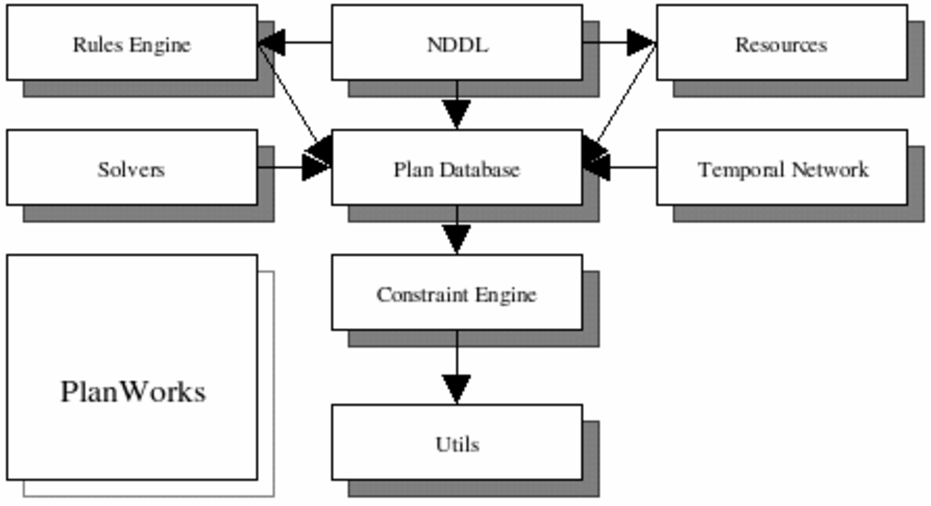
\includegraphics[width=3.5in]{./Figures/europa_architecture.pdf}
  \end{center}
%	\vspace*{-0.1in}
  \caption{\small EUROPA Modules and their dependencies.}
  \label{fig:architecture}
%  	\vspace*{-0.1in}
\end{figure}
%--

\noindent {\bf Utils module}: provides common C++ utility classes for error checking, smart pointers etc. It also includes a very useful debugging utility. Many common programming practices in EUROPA development are built on assets in this module.\\

\noindent {\bf Constraint Engine}: is the nexus for consistency management. It provides a general-purpose component-based architecture for handling dynamic constraint networks. It deals in variables and constraints. It includes an open propagation architecture making it straightforward to integrate specialized forms of local and global constraint propagation.\\

\noindent {\bf Plan Database}: adds higher levels of abstractions for tokens and objects and the interactions between them. This is the code embodiment of the EUROPA planning paradigm. It supports all services for creation, deletion, modification and inspection of partial plans. It maintains the dynamic constraint network underlying a partial�plan by delegation to the Constraint Engine and leverages that propagation infrastructure to maintain relationships between tokens and objects.\\

\noindent {\bf Solvers module}: provides abstractions to support search in line with the EUROPA planning approach. It includes a component-based architecture for Flaw Identification, Resolution and heuristics as well as an algorithm for chronological backtracking search. As additional search algorithms are implemented they will be added to this module.\\



%--
\begin{figure*}
  \begin{center}
    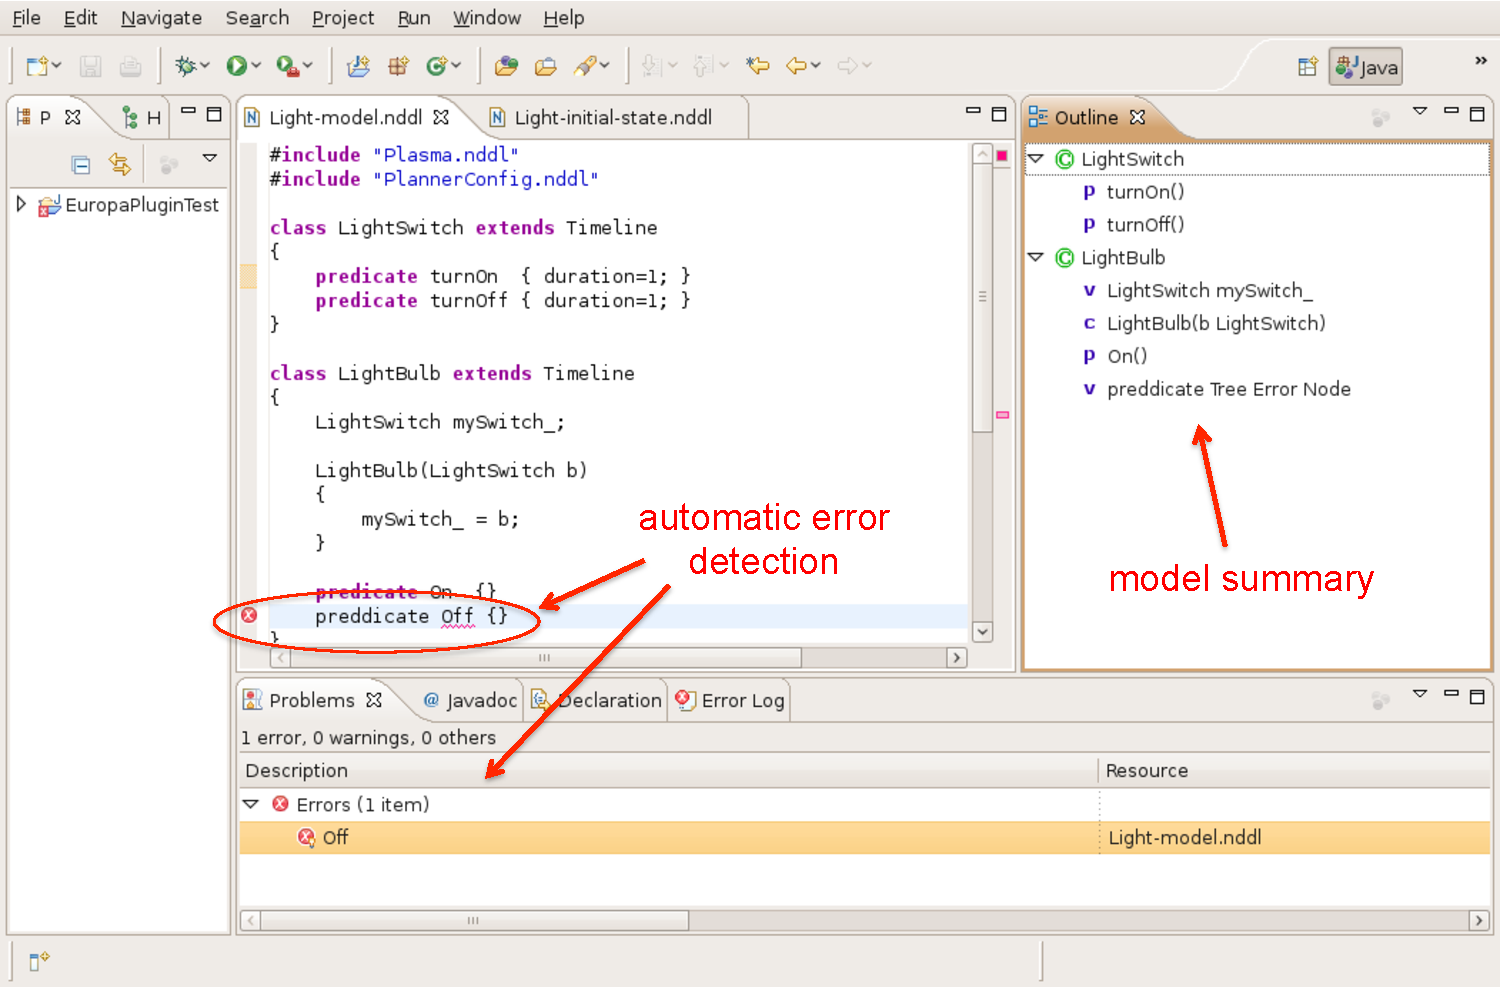
\includegraphics[width=6in]{./Figures/NDDL_editor.pdf}
  \end{center}
  \caption{\small NDDL Editor and Syntax Checker.}
  \label{fig:NDDL_editor}
\end{figure*}
%--


\noindent {\bf Rules Engine:} provides the inference capabilities based on domain rules described in the model. It is almost exclusively used to execute NDDL rules but can be extended for custom rule formats.\\

\noindent {\bf Resources module}:  provides specialized algorithms and data structures to support metric resources (e.g. battery, power bus, disk drive).
The Temporal Network module provides specialized algorithms and data structures to support efficient propagation of temporal constraints.\\

\noindent {\bf NDDL module}: provides a parser and compiler for NDDL (pronounced noodle) which is a very high-level, object-oriented, declarative domain and problem description language. This module defines the mapping from the language to the code and consequently interfaces to a number of key modules in the system.\\

\noindent {\bf PlanWorks}: is a java application for visualization and debugging of plans and planning. It is loosely coupled to the other EUROPA modules through a JNI interface.\\

From an application developer�s view-point, the modules of interest are: NDDL, Solvers and PlanWorks. These modules address modeling, search and troubleshooting respectively. Other modules will be explored in the context of making customized extensions.



%---------------------------
\section{Using EUROPA \& its Supporting Tools}

\fromM{Javier, please add in any technical elaboration that you think is useful.}\\

There are several different ways in which EUROPA can be used to to support solving a planning \& scheduling or CSP problem.


%------------------------------------
\subsection{Embed EUROPA in an Application}
EUROPA provides a makeproject script that will generate C++ and Java projects that embed EUROPA, along with simple NDDL model and initial-state files that you can then modify for your own purposes. This allow the users to perform the full application cycle of:

\begin{itemize}
\item Initialize EUROPA
\item Load/Modify model and initial state descriptions
\item Invoke a solver
\item Extract plan results from the Plan Database
\item Repeat steps 2-4 as many times as needed
\item Shutdown EUROPA
\end{itemize}

\noindent {\bf Using the C++ or JAVA API:} The PSEngine interface is the official interface for EUROPA clients, it is the recommended way to use EUROPA. This interface is very straightforward and allows you to run the entire application cycle described above. This abstraction layer will isolate your client code from most changes in the internals of the EUROPA implementation, it is also designed for easy mapping to other languages using SWIG.\\

\noindent {\bf Applications using different programming languages:} the corresponding binding for the PSEngine interface should be either already available in the EUROPA distribution, or relatively easy to add. Note that while currently only Java bindings are bundled with the EUROPA distribution, we have plans to add Python and any other languages that are popular with the EUROPA user community. This should not be too difficult given that SWIG supports multiple high-level programming languages.


%------------------
\subsection{Eclipse Plugin (SWT) for EUROPA Modeling, Solving, and Debugging}
The Eclipse plugin has two major components: (1) an editor and (2) an execution perspective. They provide the graphical interface to model, run, and analyze plans within the Eclipse development environment. The main capabilities are:

%--
\begin{figure*}
  \begin{center}
    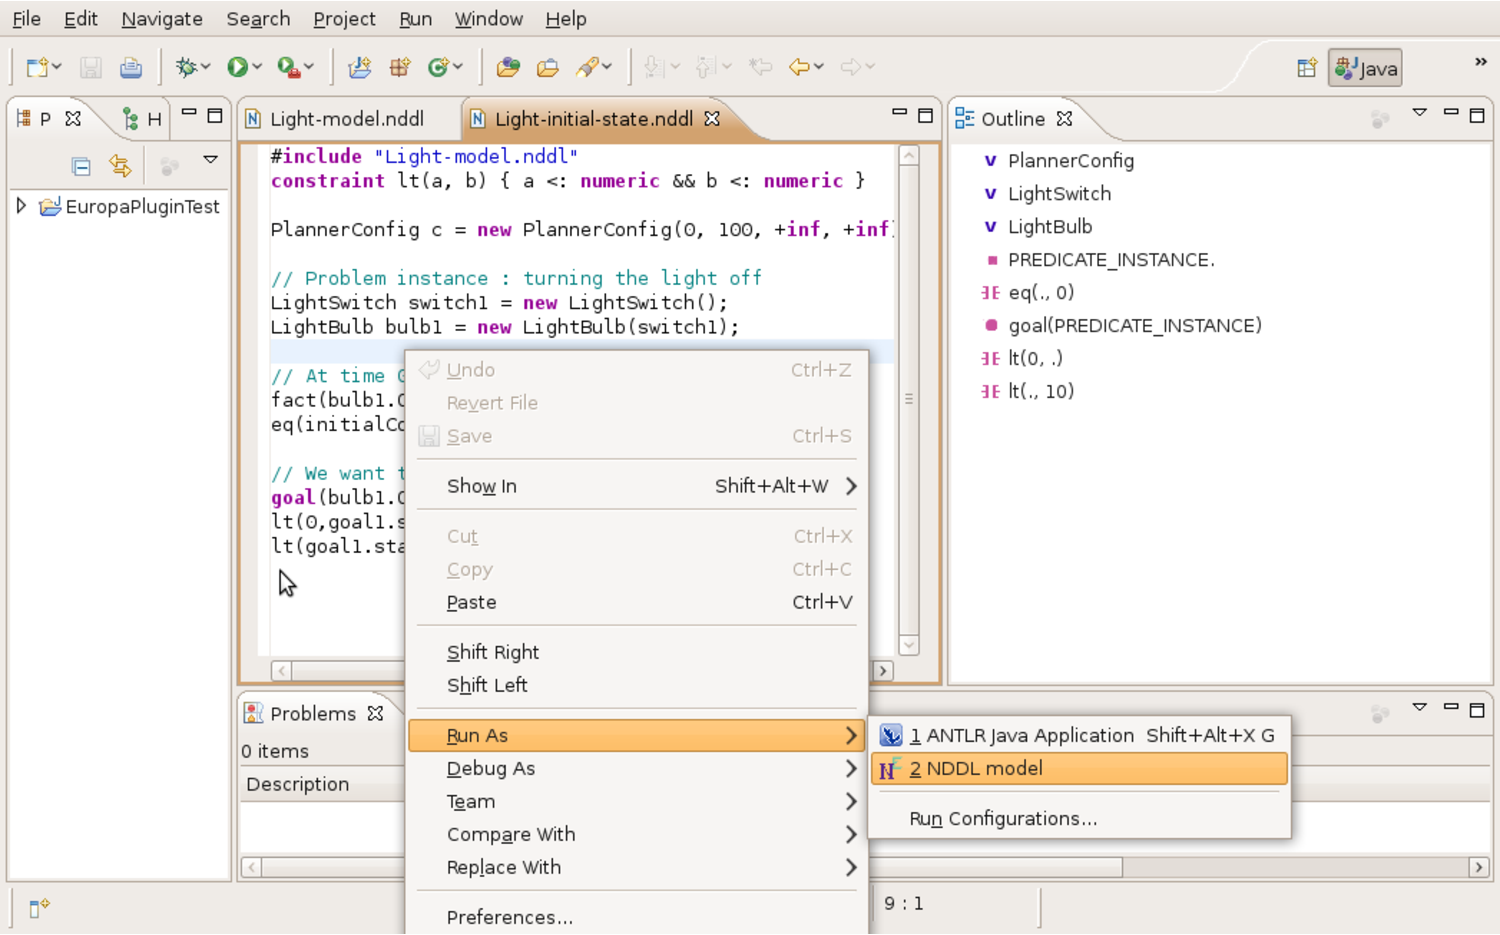
\includegraphics[width=6in]{./Figures/NDDL_runas.pdf}
  \end{center}
  \caption{\small Running a problem directly from the NDDL editor.}
  \label{fig:NDDL_runas}
\end{figure*}
%--

%--
\begin{figure*}
  \begin{center}
    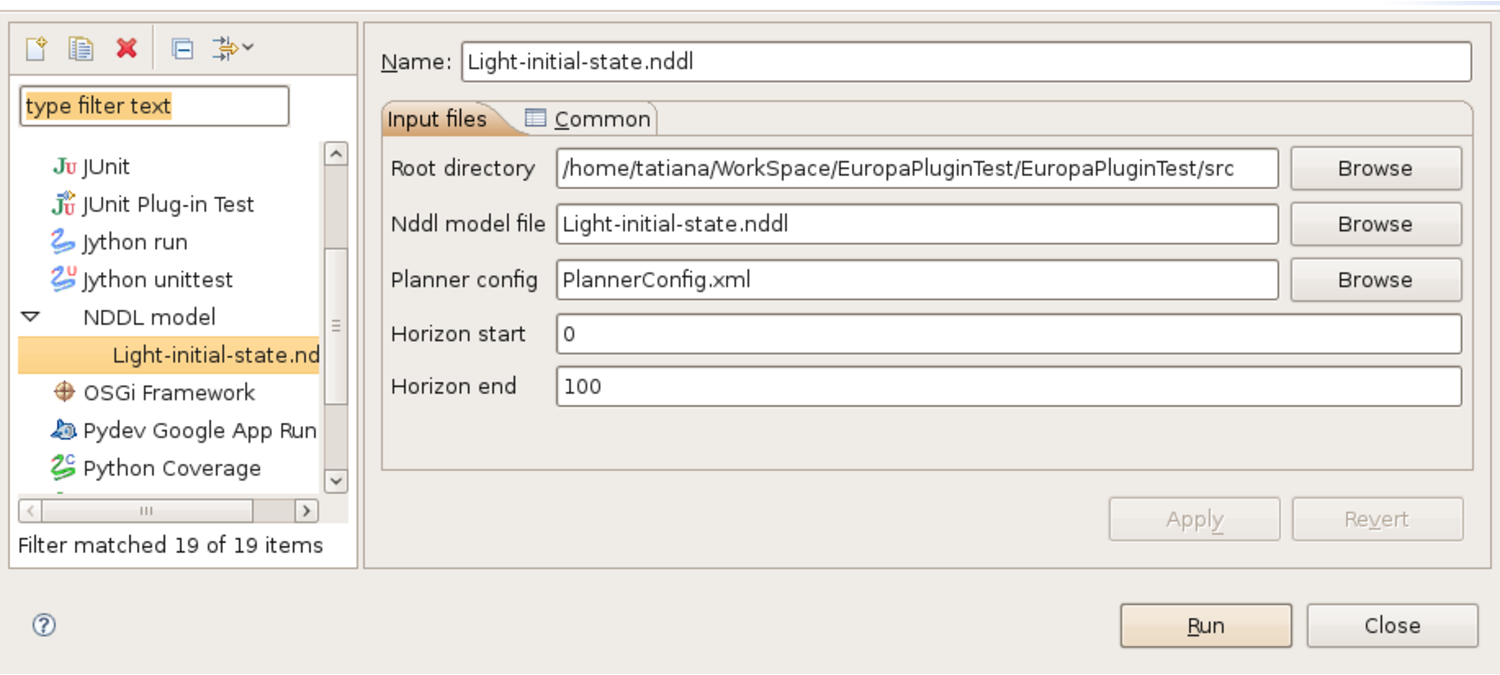
\includegraphics[width=6in]{./Figures/NDDL_runconfig.pdf}
  \end{center}
  \caption{\small Configurate a NDDL run.}
  \label{fig:NDDL_runconfig}
\end{figure*}
%--


%--
\begin{figure*}
  \begin{center}
    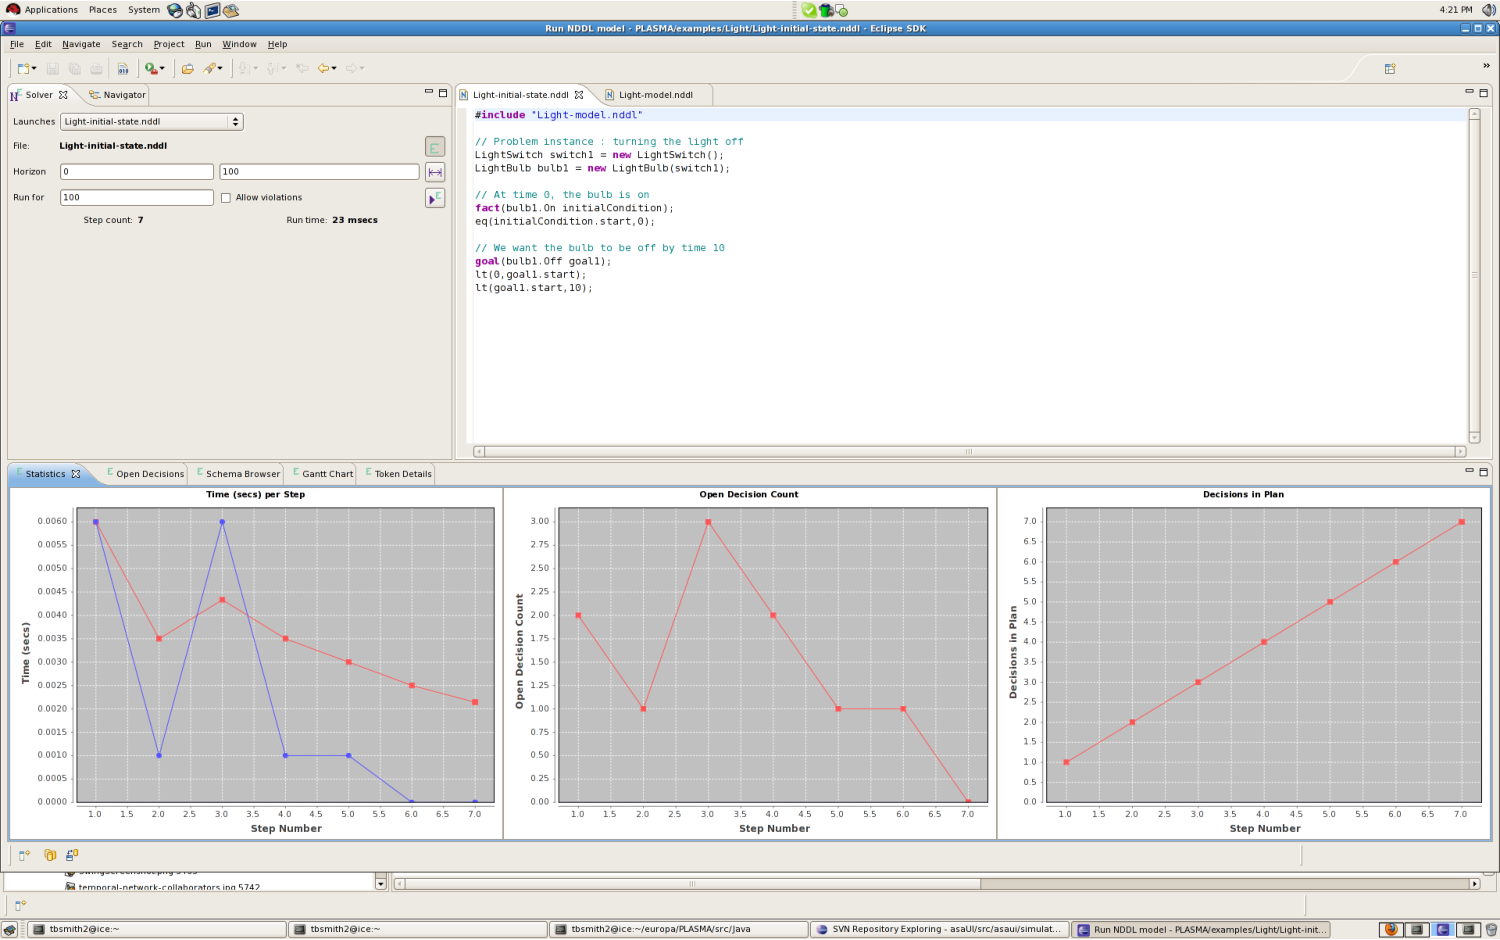
\includegraphics[width=6in]{./Figures/EclipseRunPerspective.pdf}
  \end{center}
  \caption{\small Eclipse dedicated perspective on showing information about running EUROPA}
  \label{fig:NDDL_runpers}
\end{figure*}
%--


\begin{itemize}
\item {\em NDDL Editor}: Syntax highlighting, syntax errors reporting, and linking structure to standard Outline View.
\item {\em Solver View}: Start/stop the EUROPA engine, and configure and run a solver.
\item {\em Statistics View}: Graphs of solver stats.
\item {\em Open Decision View}: View of open decisions at each step of solving.
\item {\em Schema Browser View}: View the schema for the active NDDL model.
\item {\em Gantt View}: Once a solution is found, view the plan.
\item {\em Details View}: Click on a token in the Gantt View to see it's details in this view.
\item {\em Run NDDL model perspective}: Includes all of the above components.
\end{itemize}

\noindent {\bf NDDL Graphical Model Editor:} Eclipse plugin registers a file type for ".nddl" and a default editor for it. The editor has \emph{syntax highlighting} and an \emph{outline}, which is updated every time an editor is saved. If the parser detects any errors, they are displayed as error markers in the editor. Figure~\ref{fig:NDDL_editor} shows the GUI for editing and checking the NDDL files.

Users can run EUROPA by directly invoke the \emph{Run As} action for a given NDDL file. This action shows up both in the editor and in the \emph{Package Explorer} pane. It creates a launch configuration and switches the perspective to NDDL model execution. Figure~\ref{fig:NDDL_runas} shows graphically this option. Figure~\ref{fig:NDDL_runconfig} show how to configure the run directly from within Eclipse.\\


\noindent {\bf Run NDDL Model Perspective:} The Run as NDDL model perspective is the Eclipse version of the Swing PSDesktop user interface, which was the different (earlier) implementation of the EUROPA user interface. The plugin can run multiple NDDL sessions at the same time. You can switch between them using the pulldown list. EUROPA sessions are also visible in the Debug perspective and can be killed or restarted from there. Figure~\ref{fig:NDDL_runpers} shows an example of this perspective where different aspects of modeling and execution can be visually displayed.


%-----------
\subsection{JAVA Swing UI Framework}


%--
\begin{figure*}
  \begin{center}
    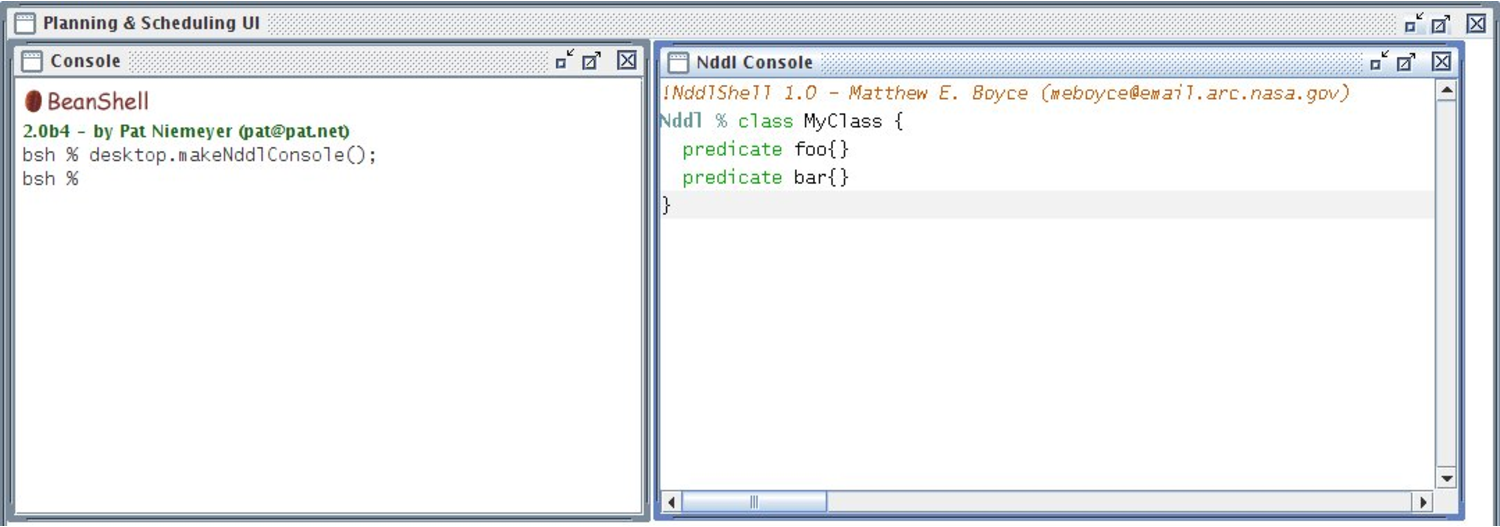
\includegraphics[width=6in]{./Figures/PSDesktop_1.pdf}
  \end{center}
  \caption{\small BeanShell and NDDL console windows}
  \label{fig:PSDesktop_start}
\end{figure*}
%--

%--
\begin{figure*}
  \begin{center}
    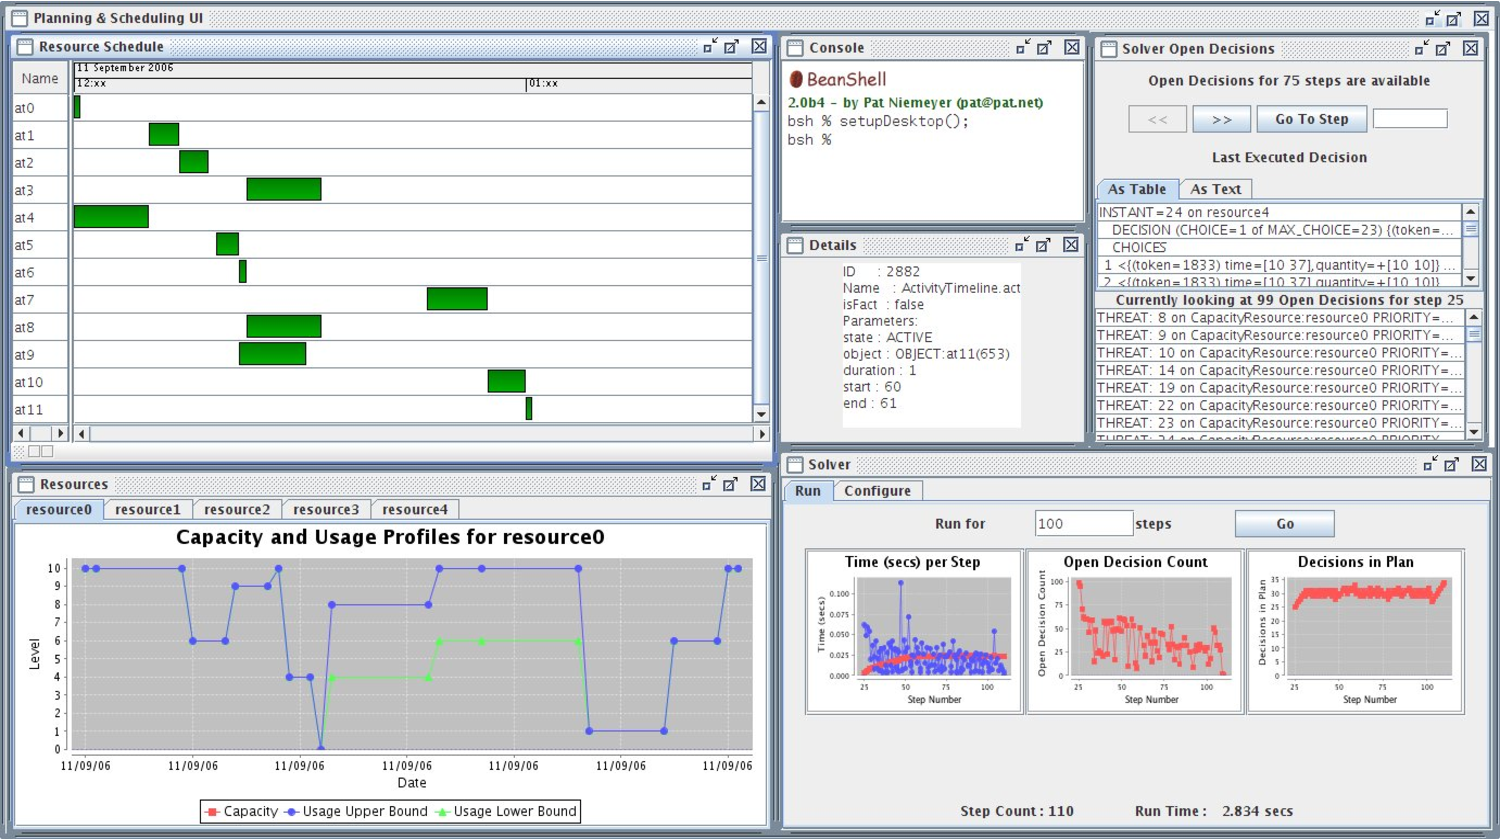
\includegraphics[width=6in]{./Figures/Example_UBO0.pdf}
  \end{center}
  \caption{\small Example of PSUI components}
  \label{fig:PSUI_exp}
\end{figure*}
%--



PSDesktop is a Java application that allows the user to drive EUROPA interactively by making use of the PSEngine client interface. It takes two arguments:

\begin{itemize}
\item To select \emph{Debug} or \emph{Optimized} version of EUROPA to run.
\item  \emph{bsh} file (optional) : filename of the \emph{BeanShell} file that is executed upon starting\footnote{BeanShell is a small, free, embeddable Java source interpreter with object scripting language features, written in Java. BeanShell dynamically executes standard Java syntax and extends it with common scripting conveniences such as loose types, commands, and method closures like those in Perl and JavaScript.}.
\end{itemize}

Figure~\ref{fig:PSDesktop_start} shows the two console windows when running PSDesktop. In the BeanShell console window you can type in Java statements that allow you to drive EUROPA interactively through its Java API. In the NDDL console you can type in NDDL statements that will be interpreted as soon as you complete a valid NDDL statement and hit enter.\\

\noindent {\em Variables exposed through BeanShell:} In the BeanShell console, you'll have access to the following variables :

\begin{itemize}
\item \emph{PSEngine}: this will give you access to the EUROPA engine, you can create a solver, query the plan database, execute NDDL scripts, in general perform any task needed to drive EUROPA to load a model and create a plan. You can also use this interface to create your own custom solver.
\item \emph{PSDesktop}: this will give you access to many utility methods to create new desktop windows, display tables of tokens, create a solver, etc.
\end{itemize}


\noindent{\em PSUI Components:} The PSUI package contains a number of components that make it easy to visualize your plan and interact with EUROPA :

\begin{itemize}
\item {\em PSGantt} : allows you to see the tokens on a timeline as a gantt chart
\item {\em PSChart} : allows you to see resource profiles as charts
\item {\em PSSolverDialog}: allows you to drive a solver interactively and see its status as it tries to achieve the goals you specified for it
\item {\em ActionDetails and ActionViolation}: allows you to easily display violation and detail information about actions in your plan as you mouse over actions in other components (for instance a gantt chart)
\end{itemize}

Figure~\ref{fig:PSUI_exp} shows an example of how different UI components within the PSUI package can be activated to assist the plan analysis.



%--
\begin{figure*}
  \begin{center}
    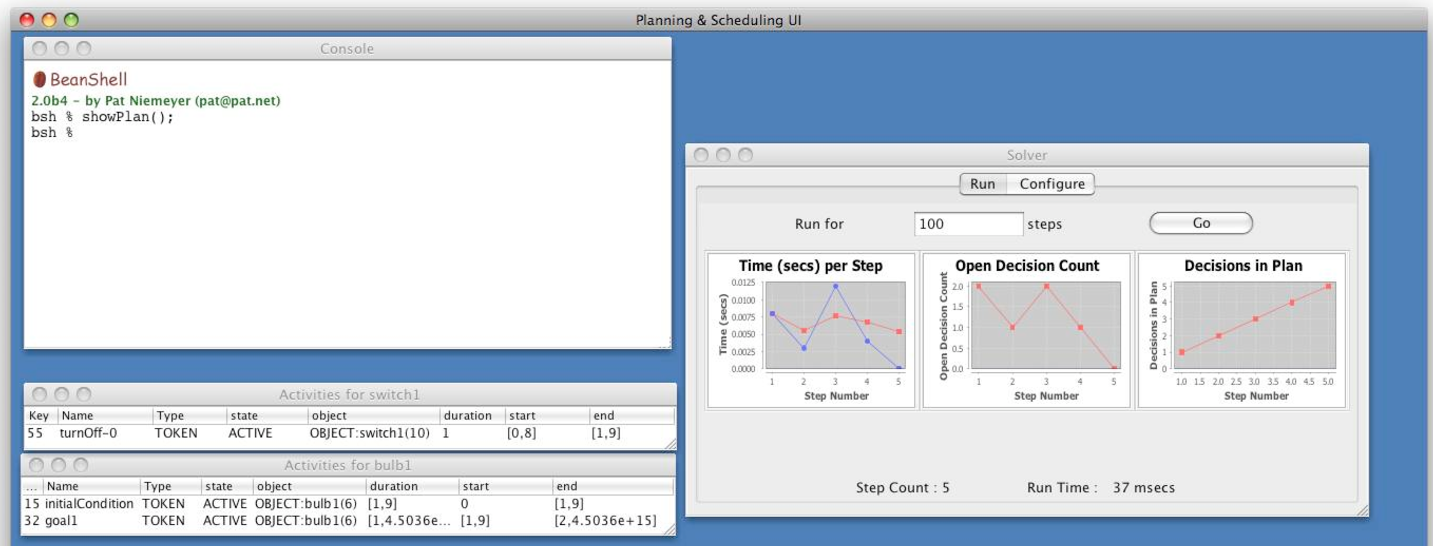
\includegraphics[width=6in]{./Figures/Examples-Light1.pdf}
  \end{center}
  \caption{\small UI example of the simple light-switch domain where the only action is to turn a light \emph{ON} or \emph{OFF}.}
  \label{fig:light_exp}
\end{figure*}
%--

%--
\begin{figure*}
  \begin{center}
    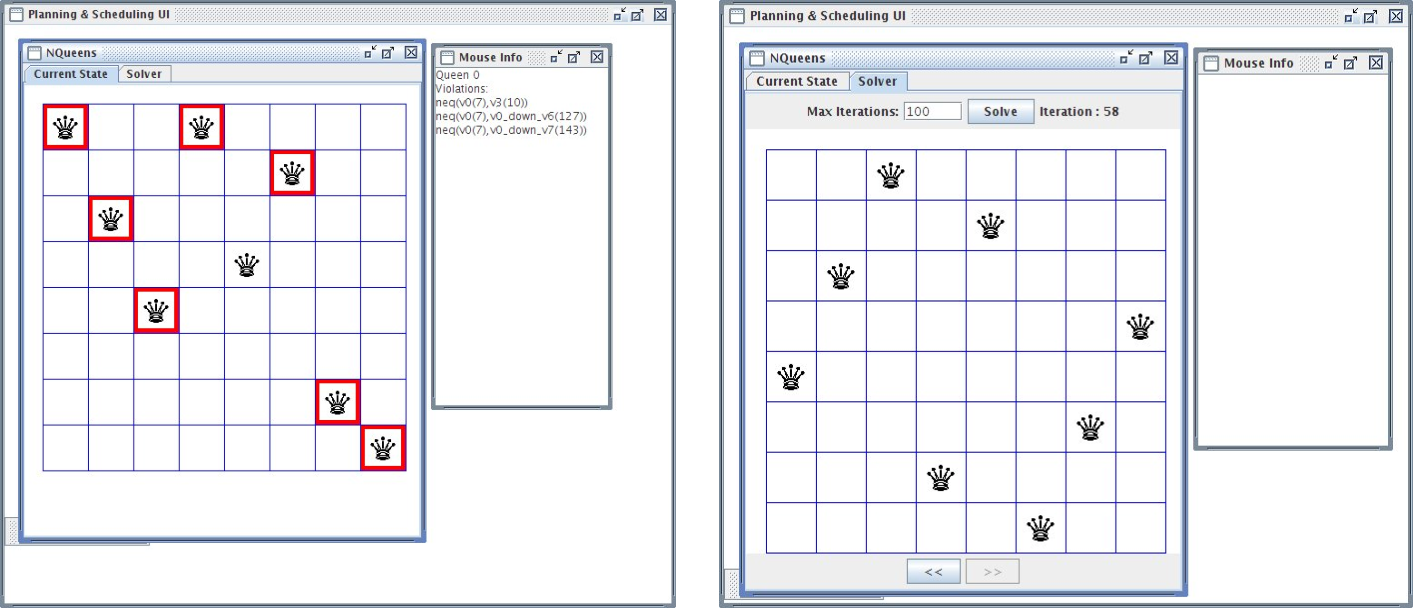
\includegraphics[width=6in]{./Figures/NQueens.pdf}
  \end{center}
  \caption{\small UI example of the representative Constraint Programming domain: NQueens}
  \label{fig:nqueens}
\end{figure*}
%--

%--
\begin{figure*}
  \begin{center}
    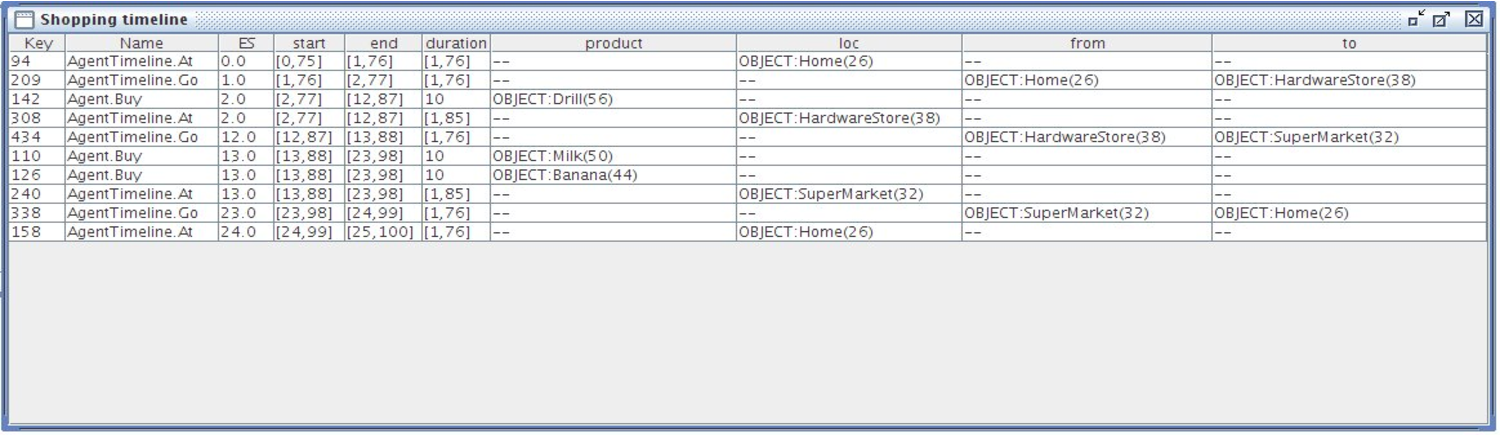
\includegraphics[width=6in]{./Figures/Examples-Shopping0.pdf}
  \end{center}
  \caption{\small UI example of the text-book \emph{shopping} planning example}
  \label{fig:shopping}
\end{figure*}
%--


%--
\begin{figure*}
  \begin{center}
    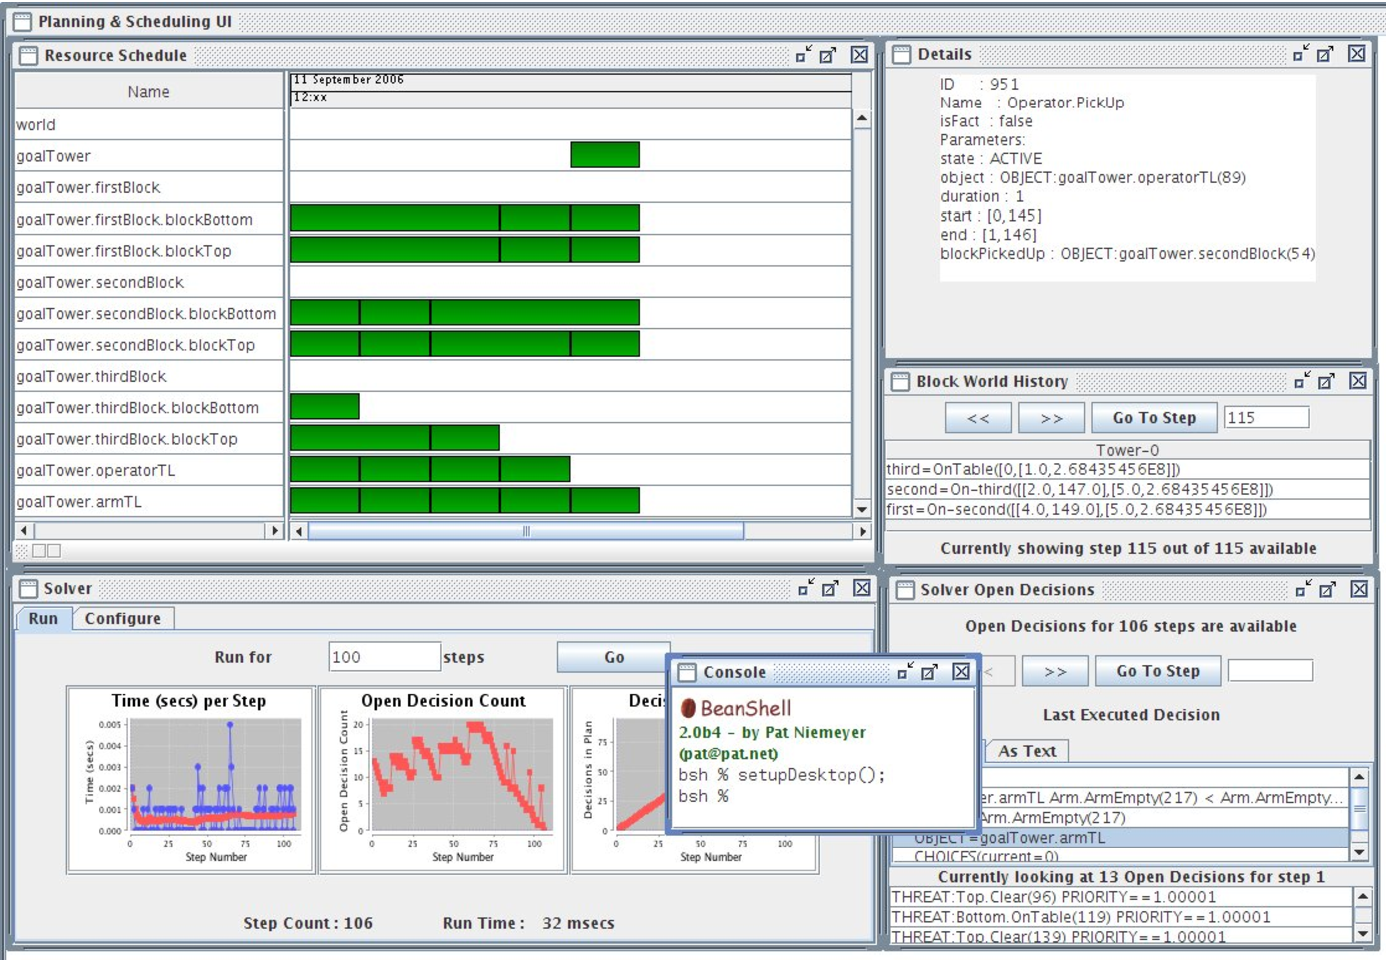
\includegraphics[width=6in]{./Figures/blocksworld.pdf}
  \end{center}
  \caption{\small UI example of the classical \emph{Blocksworld} planning domain.}
  \label{fig:blocksworld}
\end{figure*}
%--


%---------------------------
\section{Examples}

In this section, we show several examples demonstrating the flexibility of EUROPA (both its core engine and its supporting knowledge engineering tools) in solving different types of planning, scheduling, and constraint satisfaction problems. All examples shown in this section are included in the EUROPA distribution. This ranges from:

\noindent {\bf Light:} The very simple domain involving only turning the light switch ON or OFF. Figure~\ref{fig:light_exp} shows an example output analyzing the final plans. In this particular example, the intervals mean that the action or state change could happen at any point in the interval, so for instance, "lightSwitch1 is turned off at time [0,8]" means that lightSwitch1 could be turned off at time 0, or at time 1, ..., or at time 8. You can modify your model or EUROPA's configuration to generate grounded plans (where all the values are points, instead of intervals), if that's what you want for your particular application.\\

\noindent {\bf N-Queens:}  CSP's exemplary domain N-Queens (Figure~\ref{fig:nqueens}). Users can click on a chess board to move the the queens around and see the constraint violations that EUROPA computes by moving the mouse over each queen. It also provides a simple Tabu Search solver which briefly illustrates how users can build your own solver on top of EUROPA.\\

\noindent {\bf Resource Constrained Project Scheduling Problem (RCPSP):}, a  well known problem in the OR community that consists of scheduling a set of activities with temporal and resource constraints. Typically, the goal is to minimize total project duration while respecting all constraints (Figure~\ref{fig:PSUI_exp}). This example shows how users can build their own solvers on top of EUROPA.\\

\noindent {\bf Shopping}: a simple example discussed in Russel and Norvig's AI textbook, first Edition, Chapter 11 on Planning (Figure~\ref{fig:shopping}).\\

\noindent {\bf Blocksworld}: one of the most well-known planning domains. This version uses a robotic arm to build the stacks and Figure~\ref{fig:blocks world} shows a UI where you can look at the partial state of the arm and the stacks as the planner progresses towards the stated goal. Mouse over the green rectangles to see the actions over each timeline; for example, you can see the arm operator performing pick up and stack operations on the blocks. The "BlockWorld History" window shows the evolution of the stacks as the operator performs the actions from the plan on them, until it arrives to the stated goal.\\

\noindent {\bf Planetary Rover}: this is a more complex planning domain that was originated from NASA mission and has also been translated to PDDL to be used in recent IPCs. Figure~\ref{fig:rover} shows the UI result of this domain. In this figure, red and blue curves on the chart at the top-right corner bound the possible batter charge. The difference between the two is due to flexibility in the plan regarding when the navigation and sampling take place. The red curve shows the charge when they occur as soon as possible, and the blue curve shows them if everything is delayed as long as possible. The bottom window displays a gantt chart for the Rover, Navigator and Instrument timelines in this problem. Hover the mouse over any piece (green rectangle) of the gantt chart to see details displayed in the Details window. In this screenshot, the mouse was hovered over the large box on the Navigator timeline, which is an \emph{At} predicate.


%----------------------------
\section{EUROPA-related Projects}

EUROPA has been used for a variety of missions, mission-oriented research, and demonstrations, including:

\begin{itemize}
\item ATHLETE support for foot fall planning for a lunar robot
\item STAR Advanced Spaceflight Training Systems Development
\item SACE Support for operation of the International Space Station's solar arrays
\item Bedrest study at Johnson Space Center
\item Mars �09 - MSL : Support for planning and scheduling for Mars Science Laboratory Science Operations
\item Crew Planning Research project on Planning and Scheduling for space missions
\item T-REX A model based executive that integrates planning and execution for autonomous mobile robots and things that seem just like them. TREX has been deployed at sea on AUVs and on land for mobile manipulation.
\item MER Tactical Activity Planning. EUROPA is the core planning technology behind MAPGEN, a decision support tool for generating detailed activity plans on a daily basis for the MER robotic mission to Mars.
\item Mars �03: MER �Mars Exploration Rover Science Operations
\item On-board Planning and Plan Execution. EUROPA was the core planning technolgoy for deliberative and reactive planning on-board a variety of mobile robots. It has been fielded in the Atacama Desert and was the cornerstone of a 2005 milestone of human-robotic collaboration for the Collaborative Decision Systems program.
\item Mission Simulation. EUROPA was used to simulate a prospective robotic mission (LORAX) to the Antarctic for the purposes of system design evaluation.
\item Intelligent Distributed Execution Architecture (IDEA �EUROPA, EUROPA 2)
\item Earth-observing satellite scheduling project (EOS �EUROPA, EUROPA 2)
\item SOFIA flight scheduling project (SOFIA �EUROPA)
\item Contingent Planning for ROVER operations (PiCO�EUROPA 2)
\item Personal Satellite Assistant (PSA �EUROPA)
\item Spoken Interface Prototype for PSA (RIALIST �EUROPA)
\item IS Milestone (EUROPA 2, support ended in 2004)
\item CDS Milestone (EUROPA 2, currently supporting)
\item DS1: RAX �Remote Agent Experiment (original version of technology)
\end{itemize}

Outside of NASA, it has also beed used at MBARI to help control underwater autonomous vehicle and at Willow Garage with autonomous robot navigation. \fromM{Add citations to MBARI and WG work, especially the integration with T-Rex}


%-----------------------------------
\section{Conclusion and Future Work}

In this paper, we described EUROPA with concentration on its modeling and plan analysis capabilities. The main strengths of EUROPA are: (1) expressive; (2) flexible framework; (3) strong support for integrating with other applications; (4) open-source license; and (5) proven track record.

While EUROPA and its supporting tools have been going through a long period of development, we still have a long list of improvements that we want to make. Some notable improvements are: support for ANML and PDDL modeling languages,  allowing EUROPA extensions to be written in other languages, significantly improve search (especially heuristic guidance) and inference capabilities, and improve the visualization and debugging tools. Given that EUROPA is open-source software, we are welcome contribution from any planning and scheduling researcher or practitioner. \\


\noindent {\bf Acknowledgement:} EUROPA is the result of many years of research, development and deployment of constraint-based planning technology.
\begin{itemize}
\item The precursor to EUROPA was HSTS, designed and developed by Nicola Muscettola. HSTS set out the initial domain description language and essentials of the planning paradigm that became the starting point for EUROPA.
\item Ari Jonsson led the implemenation of the first version of EUROPA. Ari's team included Jeremy Frank, Paul Morris and Will Edgington, who all made valuable contributions.
\item Conor McGann led the implementation of EUROPA 2, which is a further evolution of this line of work, targeted mainly at making the technology easier to use, more efficient, easier to integrate and easier to extend. EUROPA 2's main contributors were Andrew Bachmann, Tania Bedrax-Weiss, Matthew Boyce, Patrick Daley, Will Edgington, Jeremy Frank, Michael Iatauro, Peter Jarvis, Ari Jonsson, Paul Morris, Sailesh Ramakrishnan and Will Taylor.
\item Javier Barreiro took over as the EUROPA team lead in the Fall of 2006 and has been working on it since then, improving EUROPA's technology and packaging. Javier's main in collaborators at NASA Ames are Michael Iatauro, Matthew Boyce, Tristan Smith and David Smith.
\end{itemize}

External contributors and collaborators include: Tatiana Kichkaylo, Mark Roberts, and Tony Pratkanis. Funding for this work has been provided by the NASA Intelligent Systems and Collaborative Decision Systems Programs.\\

\fromM{Need to add all relevant citations here.}


{\small
\bibliography{../../master}
\bibliographystyle{aaai}
}




\end{document}


%EOF
